\documentclass[12pt, psamsfonts]{amsart}

%-------Packages---------
\usepackage{amssymb,amsfonts}
\usepackage{fullpage}
\usepackage{todonotes}
\usepackage{physics}
\usepackage[all,arc]{xy}
\usepackage{enumerate}
\usepackage{mathrsfs}
\usepackage{theoremref}
\usepackage{graphicx}
\usepackage[bookmarks]{hyperref}

%--------Theorem Environments--------
%theoremstyle{plain} --- default
\newtheorem{thm}{Theorem}[section]
\newtheorem{cor}[thm]{Corollary}
\newtheorem{prop}[thm]{Proposition}
\newtheorem{lem}[thm]{Lemma}
\newtheorem{conj}[thm]{Conjecture}
\newtheorem{quest}[thm]{Question}

\theoremstyle{definition}
\newtheorem{defn}[thm]{Definition}
\newtheorem{defns}[thm]{Definitions}
\newtheorem{con}[thm]{Construction}
\newtheorem{exmp}[thm]{Example}
\newtheorem{exmps}[thm]{Examples}
\newtheorem{notn}[thm]{Notation}
\newtheorem{notns}[thm]{Notations}
\newtheorem{addm}[thm]{Addendum}
\newtheorem*{exer}{Exercise}

\theoremstyle{remark}
\newtheorem{rem}[thm]{Remark}
\newtheorem{rems}[thm]{Remarks}
\newtheorem{warn}[thm]{Warning}
\newtheorem{sch}[thm]{Scholium}

\DeclareMathOperator{\Hom}{Hom}
\DeclareMathOperator{\Id}{Id}
\DeclareMathOperator{\RP}{\mathbb{R}\mathbf{P}^2}

\makeatletter
\let\c@equation\c@thm
\makeatother
\numberwithin{equation}{section}

\bibliographystyle{plain}

\begin{document}

\title{Math 611 (Due 10/2)}
\author{Hidenori Shinohara}
\maketitle

\begin{exer}{(Problem 10, Chapter 1.3)}
  Find all the connected 2-sheeted and 3-sheeted covering spaces of $S^1 \vee S^1$, up to isomorphisms of covering spaces without base points.
\end{exer}

\begin{proof}
  Let $X = S^1 \vee S^1$.
  By the discussion on P.70 of the textbook, we know that $n$-sheeted covering spaces of $X$ are classified by equivalence classes of homomorphisms $\pi_1(X, x_0) \rightarrow S_n$.
  \begin{figure}
    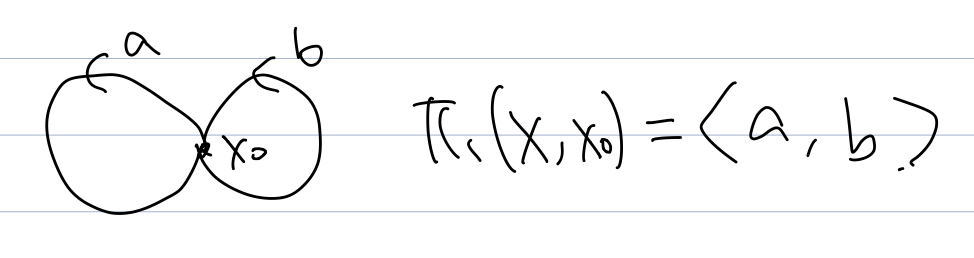
\includegraphics[width=.5\linewidth]{problem10_s1.jpeg}
    \caption{Problem 10 ($X = S^1 \vee S^1$)}
    \label{fig:problem10}
  \end{figure}
  Let $a, b$ denote paths in $X$ as in Figure \ref{fig:problem10}.
  We can identify each homomorphism $\phi$ by checking what $\phi$ maps $a$ and $b$ to.
  (Strictly speaking, $\pi_1(X, x_0)$ is generated by $[a], [b]$, but we will abuse notations by writing $a$ and $b$ instead of $[a], [b]$.)


  The following are all the cases.
  Figure \ref{fig:problem10_2_sheeted} shows the corresponding graphs.
  \begin{itemize}
    \item
      Case 1: $\phi_1(a) = \phi_1(b) = (1)$.
      The space that corresponds to this homomorphism is disconnected.
    \item
      Case 2: $\phi_2(a) = (12), \phi_2(b) = (1)$.
      This generates a connected covering space.
    \item
      Case 3: $\phi_3(a) = (1), \phi_3(b) = (12)$.
      This generates a connected covering space.
    \item
      Case 4: $\phi_4(a) = (12), \phi_4(b) = (12)$.
      This generates a connected covering space.
  \end{itemize}

  $\phi_1 \ne \phi_2$ and $(12)\phi_1(12) \ne \phi_2$, so $\phi_1$ and $\phi_2$ are not conjugates of each other.
  Similarly, $\phi_2$ and $\phi_3$ are not conjugates of each other, and neither are $\phi_1$ and $\phi_3$.

  Thus the three graphs corresponding to Case 2, 3 and 4 in Figure \ref{fig:problem10_2_sheeted} are all the 2-sheeted covering spaces of $X$.

  \begin{figure}
    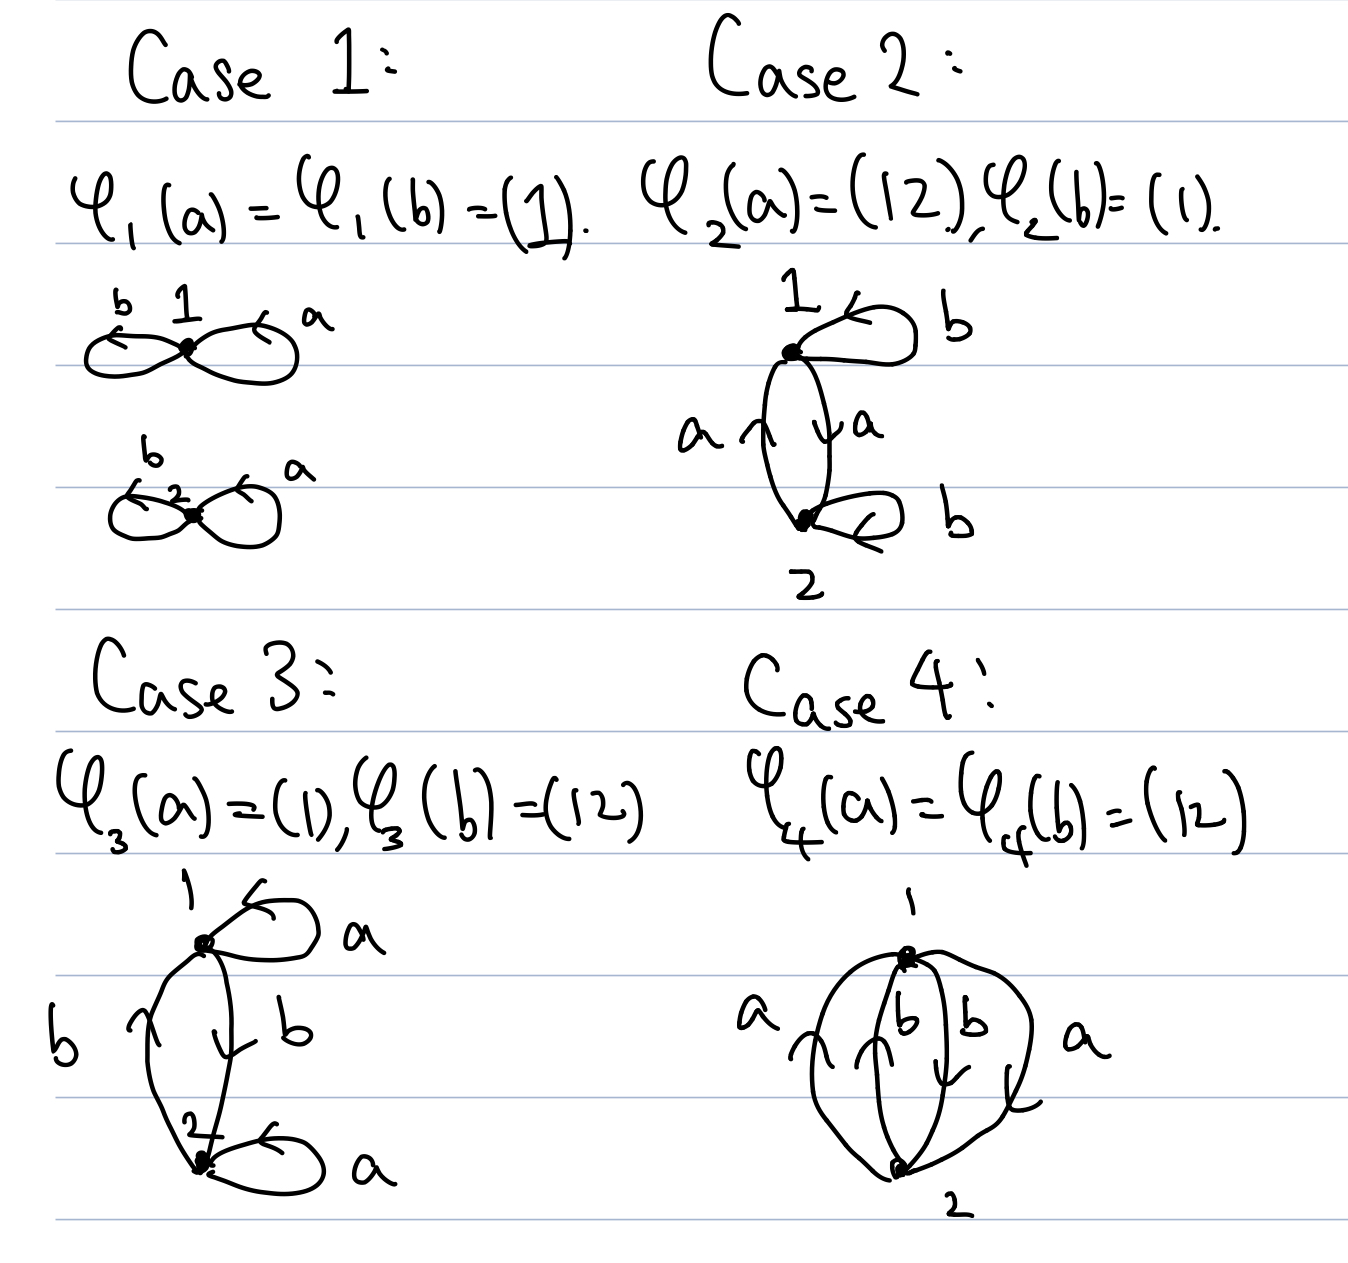
\includegraphics[width=.5\linewidth]{problem10_2_sheeted.jpeg}
    \caption{Problem 10 (2-sheeted covers)}
    \label{fig:problem10_2_sheeted}
  \end{figure}

  We will take the exact same approach for the case of 3.
  If a certain vertex is fixed in both $\phi(a)$ and $\phi(b)$, then such a vertex is disjoint from the rest of the graph.
  We will use that property to reduce the possibilities.
  \begin{figure}
    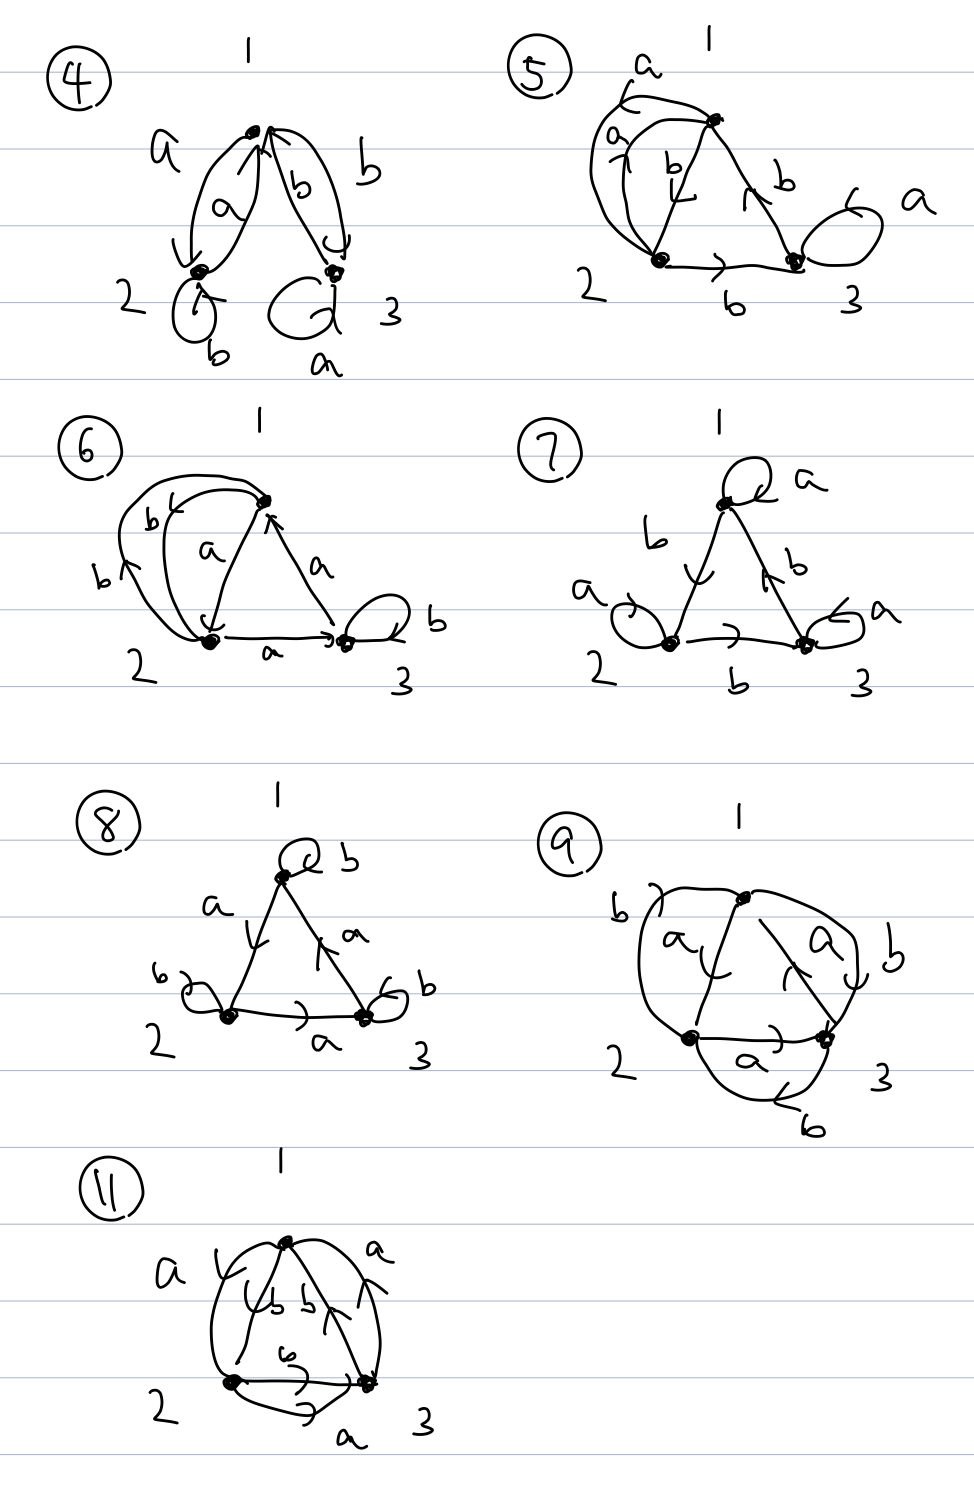
\includegraphics[width=.5\linewidth]{problem10_3_sheeted.jpeg}
    \caption{Problem 10 (3-sheeted)}
    \label{fig:problem10_3_sheeted}
  \end{figure}
  \begin{itemize}
    \item Case 1: $\phi_{1}: a \mapsto (1), b \mapsto (1)$
      The following maps are conjugates of $\phi_{1}$
      \begin{itemize}
        \item $a \mapsto (1), b \mapsto (1)$
      \end{itemize}
      This graph is not connected because every vertex is fixed.
    \item Case 2: $\phi_{2}: a \mapsto (12), b \mapsto (1)$
      The following maps are conjugates of $\phi_{2}$
      \begin{itemize}
        \item $a \mapsto (23), b \mapsto (1)$
        \item $a \mapsto (13), b \mapsto (1)$
        \item $a \mapsto (12), b \mapsto (1)$
      \end{itemize}
      This graph is not connected because vertex 3 is fixed.
    \item Case 3: $\phi_{3}: a \mapsto (1), b \mapsto (12)$
      The following maps are conjugates of $\phi_{3}$
      \begin{itemize}
        \item $a \mapsto (1), b \mapsto (12)$
        \item $a \mapsto (1), b \mapsto (23)$
        \item $a \mapsto (1), b \mapsto (13)$
      \end{itemize}
      This is the same as Case 2.
    \item Case 4: $\phi_{4}: a \mapsto (12), b \mapsto (13)$
      The following maps are conjugates of $\phi_{4}$
      \begin{itemize}
        \item $a \mapsto (13), b \mapsto (12)$
        \item $a \mapsto (12), b \mapsto (23)$
        \item $a \mapsto (12), b \mapsto (13)$
        \item $a \mapsto (13), b \mapsto (23)$
        \item $a \mapsto (23), b \mapsto (12)$
        \item $a \mapsto (23), b \mapsto (13)$
      \end{itemize}
      See Figure \ref{fig:problem10_3_sheeted}.
    \item Case 5: $\phi_{5}: a \mapsto (12), b \mapsto (123)$
      The following maps are conjugates of $\phi_{5}$
      \begin{itemize}
        \item $a \mapsto (23), b \mapsto (123)$
        \item $a \mapsto (12), b \mapsto (123)$
        \item $a \mapsto (12), b \mapsto (132)$
        \item $a \mapsto (13), b \mapsto (132)$
        \item $a \mapsto (13), b \mapsto (123)$
        \item $a \mapsto (23), b \mapsto (132)$
      \end{itemize}
      See Figure \ref{fig:problem10_3_sheeted}.
    \item Case 6: $\phi_{6}: a \mapsto (123), b \mapsto (12)$
      The following maps are conjugates of $\phi_{6}$
      \begin{itemize}
        \item $a \mapsto (123), b \mapsto (13)$
        \item $a \mapsto (132), b \mapsto (12)$
        \item $a \mapsto (132), b \mapsto (23)$
        \item $a \mapsto (132), b \mapsto (13)$
        \item $a \mapsto (123), b \mapsto (12)$
        \item $a \mapsto (123), b \mapsto (23)$
      \end{itemize}
      See Figure \ref{fig:problem10_3_sheeted}.
    \item Case 7: $\phi_{7}: a \mapsto (1), b \mapsto (123)$
      The following maps are conjugates of $\phi_{7}$
      \begin{itemize}
        \item $a \mapsto (1), b \mapsto (132)$
        \item $a \mapsto (1), b \mapsto (123)$
      \end{itemize}
      See Figure \ref{fig:problem10_3_sheeted}.
    \item Case 8: $\phi_{8}: a \mapsto (123), b \mapsto (1)$
      The following maps are conjugates of $\phi_{8}$
      \begin{itemize}
        \item $a \mapsto (132), b \mapsto (1)$
        \item $a \mapsto (123), b \mapsto (1)$
      \end{itemize}
      See Figure \ref{fig:problem10_3_sheeted}.
    \item Case 9: $\phi_{9}: a \mapsto (123), b \mapsto (132)$
      The following maps are conjugates of $\phi_{9}$
      \begin{itemize}
        \item $a \mapsto (123), b \mapsto (132)$
        \item $a \mapsto (132), b \mapsto (123)$
      \end{itemize}
      See Figure \ref{fig:problem10_3_sheeted}.
    \item Case 10: $\phi_{10}: a \mapsto (23), b \mapsto (23)$
      The following maps are conjugates of $\phi_{10}$
      \begin{itemize}
        \item $a \mapsto (12), b \mapsto (12)$
        \item $a \mapsto (23), b \mapsto (23)$
        \item $a \mapsto (13), b \mapsto (13)$
      \end{itemize}
      Vertex 1 is disconnected from the rest of the graph since it is fixed.
    \item Case 11: $\phi_{11}: a \mapsto (123), b \mapsto (123)$
      The following maps are conjugates of $\phi_{11}$
      \begin{itemize}
        \item $a \mapsto (132), b \mapsto (132)$
        \item $a \mapsto (123), b \mapsto (123)$
      \end{itemize}
      See Figure \ref{fig:problem10_3_sheeted}.
  \end{itemize}
  Since there are 6 elements in $S_3$, there are 36 possible homomorphisms.
  The list above contains all of them.
  Therefore, Figure \ref{fig:problem10_3_sheeted} lists all the possible 3-sheeted covers.
\end{proof}

\begin{exer}{(Problem 11, Chapter 1.3)}
  Construct finite graphs $X_1$ and $X_2$ having a common finite-sheeted covering space $\tilde{X}_1 = \tilde{X}_2$, but such that there is no space having both $X_1$ and $X_2$ as covering spaces.
\end{exer}

\begin{proof}
  Figure \ref{fig:problem11} shows $X_1, X_2$ and $\tilde{X}_1 = \tilde{X}_2$.
  \begin{figure}
    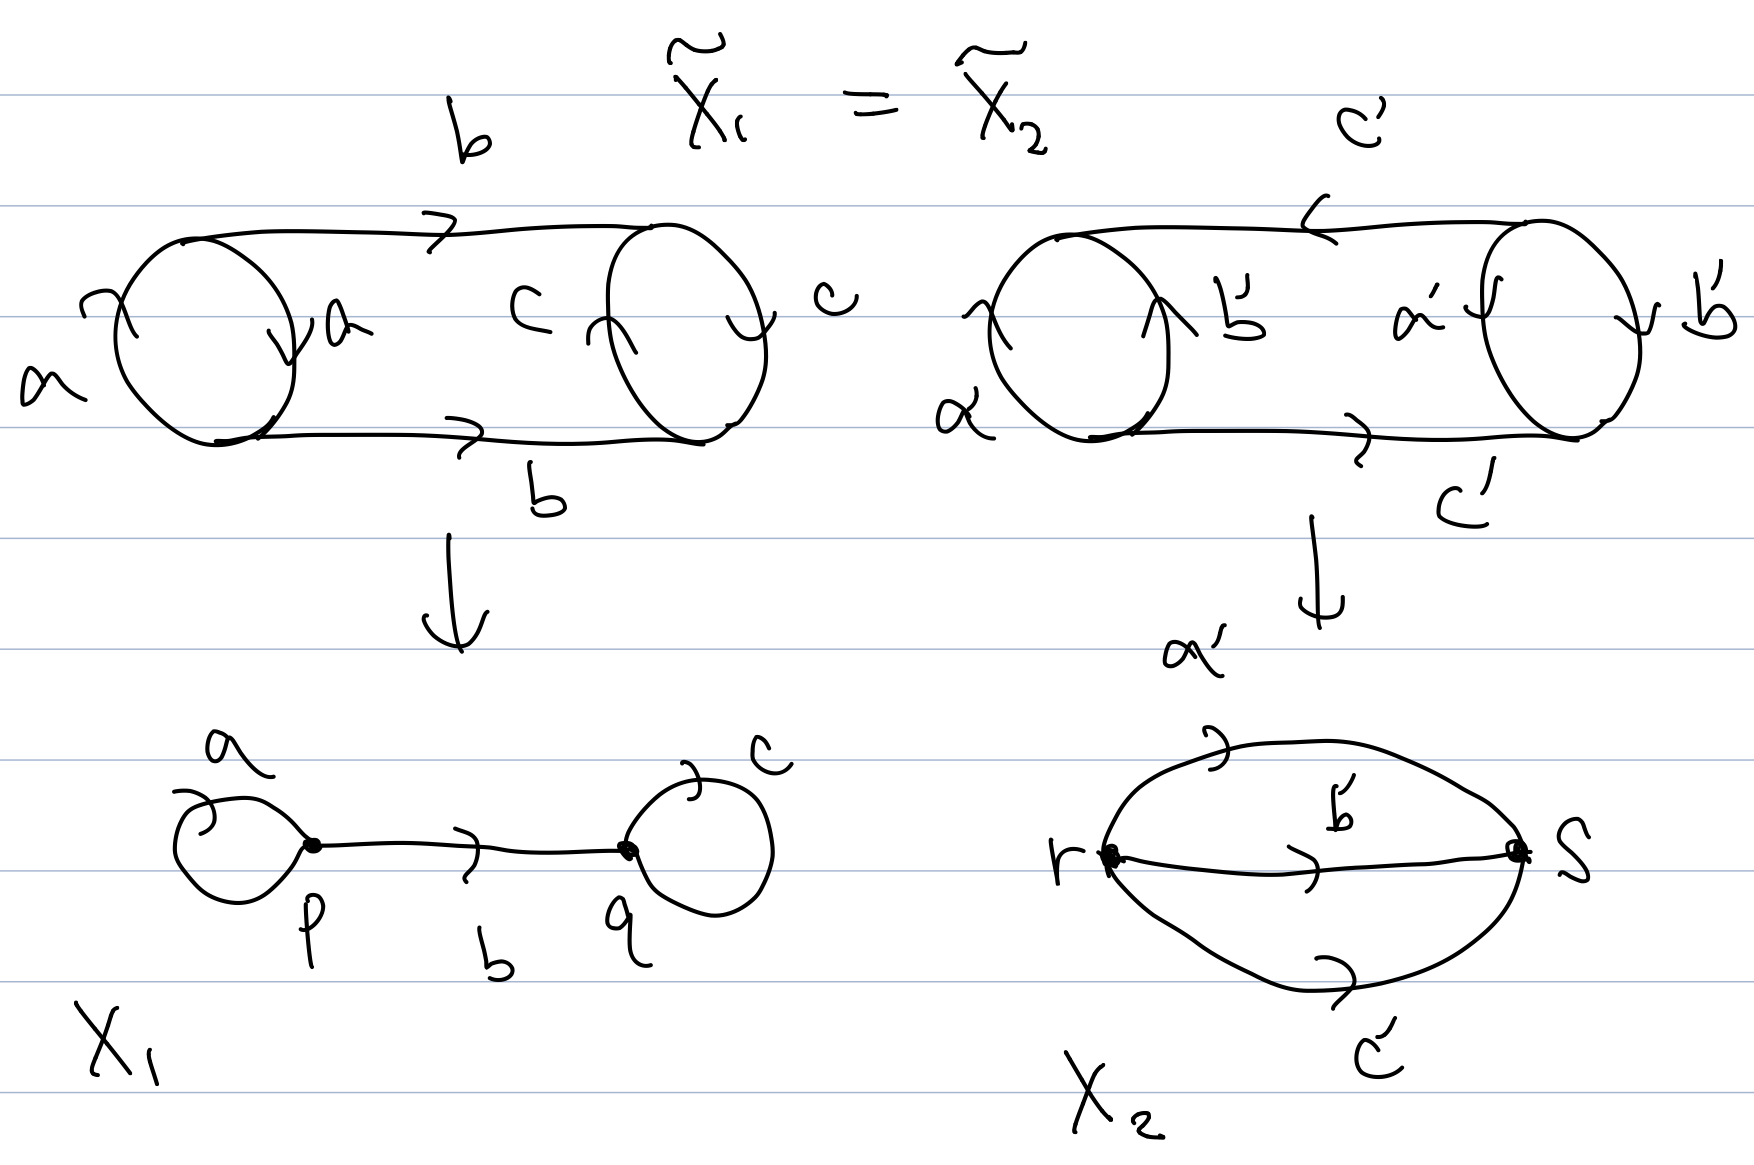
\includegraphics[width=.5\linewidth]{problem11.jpeg}
    \caption{Problem 11}
    \label{fig:problem11}
  \end{figure}
  
  We claim that there exists no space having both $X_1$ and $X_2$ as covering spaces.
  On the contrary, suppose there exists such a space $X$ with covering maps $p_1: X_1 \rightarrow X, p_2: X_2 \rightarrow X$.
  Then every point in $X$ must have a neighborhood that homeomorphic to an open subset of $X_1$.
  Since $X_1$ is a graph, that means $X$ is locally a line and a vertex with edges.
  In other words, $X$ must be a graph.

  There must exist a neighborhood of $p_1(p)$ and a neighborhood of $p$ such that they are homeomorphic.
  Since $p$ is a vertex of degree 3, $p_1(p)$ must be a vertex of degree 3 as well.
  Similarly, $p_1(q)$ must be a vertex of degree 3 as well.

  Since $p, q$ are the only vertices of $X_1$, $X$ contains at most two vertices and their degrees must be 3.
  Since the sum of degrees of all vertices must be even from elementary graph theory, $X$ must contain two vertices of degree 3.

  If $X$ only consists of loops, then the degree of each vertex will be even.
  Thus the two vertices must be joined by at least one edge.
  Then if one vertex has a loop, the other must have a loop as well in order to have degree 3.
  If there exists another edge joining the two vertices, there must be a third one in order for the two vertices to have degree 3.
  Therefore, $X_1, X_2$ are the only graphs with two vertices of degree 3.

  Suppose that $X_1$ is a covering space of $X_2$ with a covering map $f: X_1 \rightarrow X_2$.
  Without loss of generality, $f(p) = r, f(q) = s$.
  Consider the path $a'$ in $X_2$.
  Lifting $a'$ to $X_1$ will result in a path from $p$ to $q$.
  This implies that $f$ maps points on the path $b$ into points on a path $a'$.
  
  Now consider the path $b'$ in $X_2$.
  Lifting $b'$ to $X_1$ will again result in a path from $p$ to $q$.
  This implies that $f$ maps points on the path $b$ into points on a path $b'$.

  This implies that every point on the path $b$ must be mapped to $r$ or $s$.
  This is a contradiction because $f$ is continuous and $\{ b(t) \mid t \in [0, 1] \}$ is connected, but $\{ r, s \}$ is disconnected.

  Thus $X_1$ is not a covering space of $X_2$.

  Similarly, suppose that $X_2$ is a covering space of $X_1$ with a covering map $g: X_2 \rightarrow X_1$.
  Without loss of generality, $g(r) = p, g(s) = q$.
  This implies $g^{-1}(p) = \{ r \}$, so the number of sheets is 1.
  In other words, $g$ is injective.
  Consider the path $a$ in $X_1$.
  Lifting $a$ to $X_2$ results into a loop based at $r$.
  Since $a: I \rightarrow X_1$ is injective, $\tilde{a}: I \rightarrow X_2$ is injective since $g \circ \tilde{a} = a$.
  Then $\tilde{a}(t) = s$ for some $t \in [0, 1]$, so $a(t) = g(\tilde{a}(t)) = g(s) = q$.
  However, $q$ is not a point on $a$.
  This is a contradiction, so $X_2$ is not a covering space of $X_1$.

  Hence, there exists no space that has both $X_1$ and $X_2$ as covering spaces.
\end{proof}

\begin{exer}{(Problem 14, Chapter 1.3)}
  Find all the connected covering spaces of $\RP \vee \RP$.
\end{exer}

\begin{proof}
  Let $X = \RP \vee \RP$.
  By Theorem 1.38 of the textbook, it suffices to check all the conjugacy classes of subgroups of $\pi_1(X, x_0)$.

  Since $\pi_1(\RP) = \langle a \mid a^2 \rangle$, $\pi_1(X, x_0) = \langle a, b \mid a^2 = b^2 = e \rangle$ by Van Kampen.
  Since $a^2 = b^2 = e$, we can express each element in $\pi_1(X, x_0)$ uniquely as a word which alternates $a, b$.

  Here are all the conjugacy classes of subgroups:
  \begin{enumerate}
    \item
      Conjugacy class represented by $\ev{e}$.
    \item
      Conjugacy class represented by $\ev{a}$.
      This conjugacy class contains $\ev{bab}, \ev{ababa}, \ev{bababab}, \cdots$.
    \item
      Conjugacy class represented by $\ev{b}$.
      This conjugacy class contains $\ev{aba}, \ev{babab}, \ev{abababa}, \cdots$.
    \item
      Conjugacy class represented by $\ev{(ab)^k}$ for each $k \in \mathbb{N}$.
      There are no other elements in these conjugacy classes.
    \item
      Conjugacy class represented by $\ev{a, w}$ for each word $w$ that starts and ends with $b$,
      For each $w$, $\ev{bab, bwb}, \ev{ababa, abwba}, \cdots$ are the elements in the conjugacy class of $\ev{a, w}$.
      Each conjugacy class of this type contains finitely many elements.
      For instance, when $w = bababab$, $\ev{a, bababab}, \ev{bab, ababa}, \ev{ababa, bab}, \ev{bababab, a}$ are the only elements in this class.
  \end{enumerate}

  Figure \ref{fig:problem14} shows covering spaces corresponding to each conjugacy class.
  \begin{figure}
    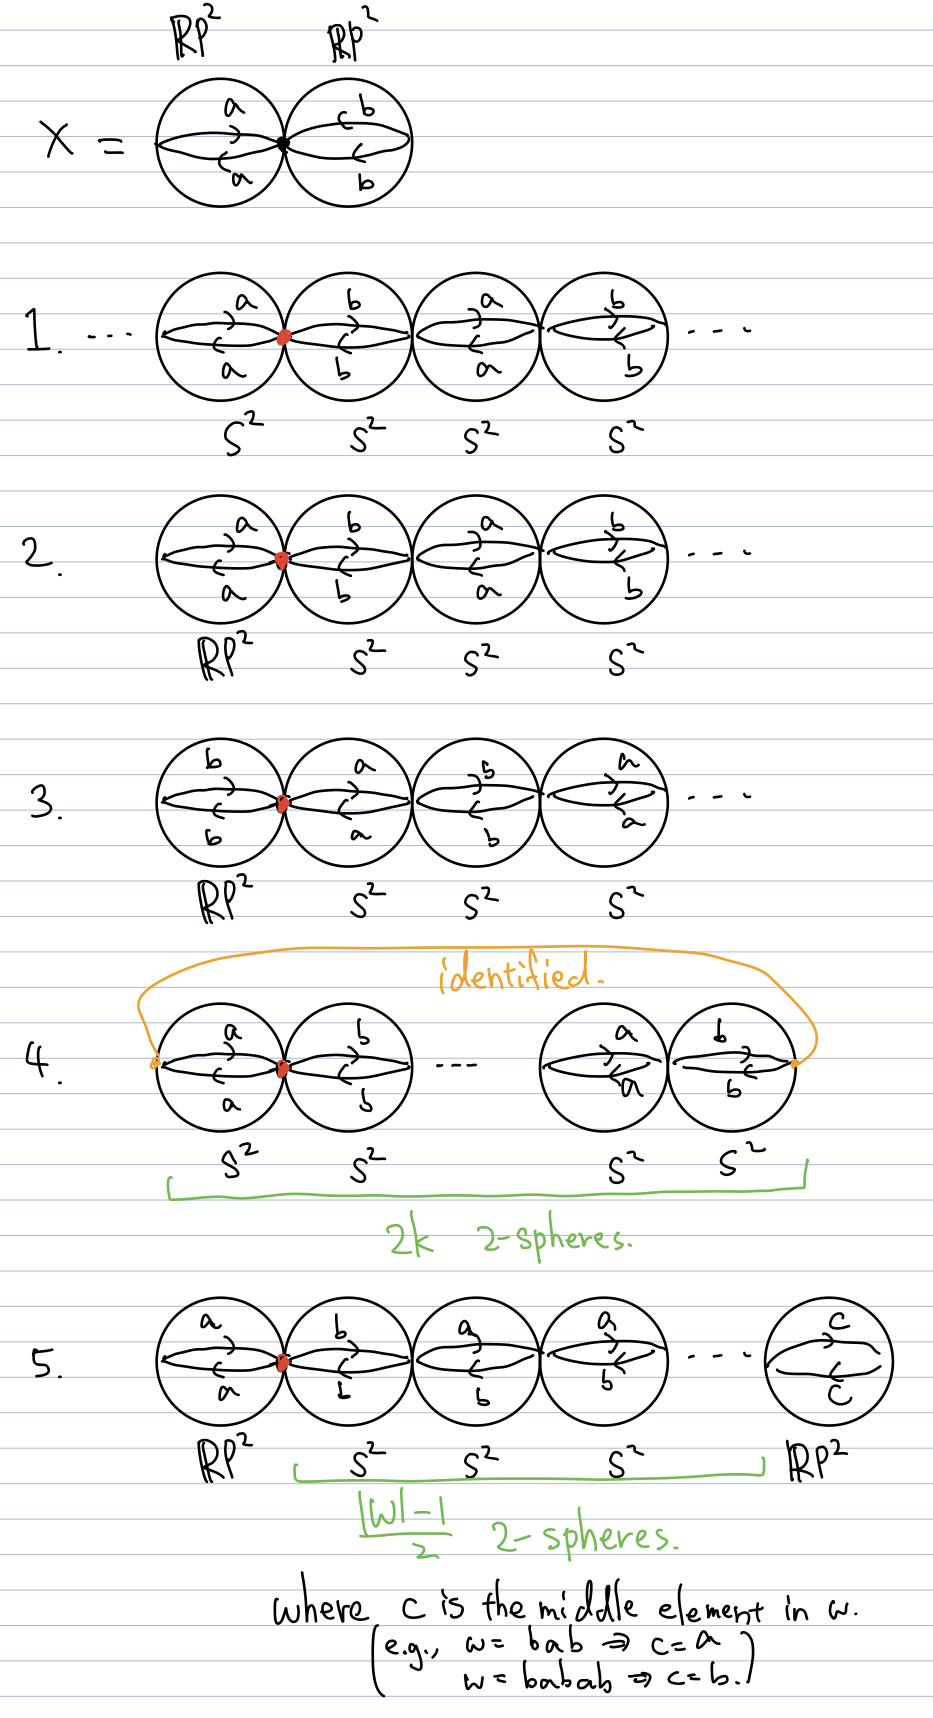
\includegraphics[width=.5\linewidth]{problem14_rp2.jpeg}
    \caption{Problem 14}
    \label{fig:problem14}
  \end{figure}

  We will prove that we have listed all the conjugacy classes, and that there are exactly 5 classes.
  \begin{itemize}
    \item
      \todo[inline]{
        All classes?
      }
    \item
      \todo[inline]{
        Different?
      }
  \end{itemize}
\end{proof}

\end{document}


